% LaTeX Sourcode

% Präambel
% Parameter von \documentclass
% https://texblog.org/2013/02/13/latex-documentclass-options-illustrated/
\documentclass[12pt,pdftex,parskip=half]{article}

% Diese Datei enthält sämtliche zusätzlich eingebundenen Pakete

% URLs mit Zeilenumbruch ermöglichen
% \usepackage[hyphens]{url}

% PDF Dokumenteneigenschaften - Hyperref ermöglicht Meta-Informationen in der PDF
% https://www.namsu.de/Extra/pakete/Hyperref.html
% Links werden im Dokument schwarz dargestellt
\usepackage[pdftitle={Seminararbeit Containerisierung vs. Virtualisierung},pdfsubject={Virtualisierung und Containerisierung},pdfauthor={Danny Langenbach},pdfkeywords={VoIP, Security, Risiken,SBC},pdfstartview=FitH,colorlinks=true,linkcolor=black,urlcolor=black,citecolor=black]{hyperref}

% https://tex.stackexchange.com/questions/3033/forcing-linebreaks-in-url
% https://tex.stackexchange.com/a/3034
% https://tex.stackexchange.com/a/10419
\PassOptionsToPackage{hyphens}{url}\usepackage{hyperref}

% Komplette PDFs einbinden
\usepackage{pdfpages}

% main=ngerman legt die Hauptsprache des Dokuments auf Neue Deutsche Rechtschreibung fest
% (Umlaute, Datum etc)
% englisch erlaubt es einzelne Abschnitte in Englisch zu definieren
\usepackage[main=ngerman, english]{babel}
\usepackage[T1]{fontenc}
\usepackage[utf8]{inputenc}  

% Für das Euro-Symbol
% \usepackage{eurosym}  \DeclareUnicodeCharacter{20AC}{\euro}

% Graphix ermöglicht die Einbindung von .jpeg,.jpg,.png usw.
\usepackage{graphicx}

% Kopzeile und Stil
\usepackage{fancyhdr}

\usepackage{caption}
% Fußnote
\usepackage{footmisc}

% Um das Abbildungsverzeichnis ins Inhaltsverzeichnis aufzunehmen
% Nottoc verhindert das sich das Inhaltsverzeichnis selbst als Inhalt nennt
% https://tex.stackexchange.com/a/297985
\usepackage[nottoc]{tocbibind}
% https://texblog.org/2013/04/29/latex-table-of-contents-list-of-figurestables-and-some-customizations/#totoc

% Package für Gesamtseitenzahl
\usepackage{lastpage}

% tabularx für Tabellen
\usepackage{tabularx}

% Für Blindtext
\usepackage{lipsum}

% Zitate APA Style - 6. Version
% Muss auskommentiert werden, wenn IEEEtran verwendet werden soll
% \usepackage{apacite}

% Für das Abkürzungsverzeichnis
% Ermöglicht die Verwendung von \acs im Text und gibt nur verwendete Abkürzungen im Glossar aus
% \usepackage[printonlyused,withpage]{acronym}
% printonlyused = Nur verwendete Acronyme angeben
% WithPage = Seite der Abkürzung im Dokument

% nopostdot = Kein Punkt nach der Abkürzung
% nonumberlist = Keine Seitenzahlen ausgeben, wo die Abkürzungen verwendet werden.
% toc = true nimmt Eintrag ins Inhaltsverzeichnis auf, ohne Notwendigkeit von \addcontentsline
% siehe https://tex.stackexchange.com/a/156742
% \usepackage[acronym,toc=true]{glossaries}
\usepackage[acronym,toc=true]{glossaries}

% \usepackage{xparse}

% Für mehrzeilige Kommentare
\usepackage{verbatim}

% Für Textoverlays wie z.B. "Entwurf" oder "Vertraulich"
% Gestaltung des Wasserzeichens unter /Layout/Wasserzeichen
% \usepackage[firstpage]{draftwatermark} - Wasserzeichen nur auf der ersten Seite
% \usepackage[nostamp]{draftwatermark} - Kein Wasserzeichen irgendwo im Dokument
% \usepackage{draftwatermark}
% Zeilenabstände
%\usepackage[onehalfspacing]{setspace}

% Zeilenabstand global 1.5-zeilig und vorher kein Einzug
\setlength{\parindent}{0pt}  \linespread{1.5}

% Zeilenabstand nach Absatz
\setlength{\parskip}{6pt}
% Kopfzeilenformatierung

% AtBeginDocument = Das globale Layout von Geometry gilt auch für Kopf-  und Fußzeile

\AtBeginDocument{

%\renewcommand{\headrulewidth}{0.4pt}
%\renewcommand{\sectionmark}[1]{\markboth{#1}{}} % set the \leftmark
% \renewcommand*\sectionmarkformat{} % keine Nummerierung im Kopf

%\RenewDocumentCommand{\section}{som}{
%  \IfBooleanTF{#1}
%   {% there's a *
%    \CLASSsection*{#3}\markboth{#3}{}
%   }
%   {% no *
%    \IfNoValueTF{#2}
%     {% no opt arg
%      \CLASSsection{#3}%
%     }
%     {% opt arg
%      \CLASSsection[#2]{#3}
%     }
%   }
% }

% fix \tableofcontents
% \renewcommand{\tableofcontents}{%
%  \section*{\contentsname}%
%  \@starttoc{toc}%
%}

% Rechter Header = leer
% \leftmark = Aktueller Abschnitt
\fancyhead[R]{}

% Mittlerer Header = Aktuelle Seite
\fancyhead[C]{\nouppercase{\thepage}}
%\fancyheadoffset[C]{1cm}

% Linker Header = leer
\fancyhead[L]{}
% \fancyheadoffset[R]{1cm}

}
% Layout der Fußzeile
% Fußzeile ist leer

% Fußzeilenformatierung
% \renewcommand{\footrulewidth}{0.4pt}

% Linke Spalte
\lfoot{} 

% Mittlere Spalte
% \cfoot{\small  \today}
\cfoot{}

% Rechte Spalte 
% \rfoot{\normalfont\small Seite \thepage / \ref{TotPages}}
\rfoot{}
% Seitengestaltung und Abstände
\usepackage[a4paper,left=40mm,right=20mm,bottom=20mm,top=40mm,bindingoffset=0mm,includeheadfoot]{geometry}
% includeheadfoot  = Layout greift auch für Kopf und Fußzeile. 
% includefoot = Nur für Fußzeile
% includehead = Nur für Kopfzeile
%Für Farben im allgemeinen
\usepackage{xcolor} 

% RGB zu CYMK
% https://codebeautify.org/rgb-to-cmyk-converter

%Definition der Firmenfarben
\definecolor{effexxrot}{cmyk}{0.0000,0.9736,0.9163,0.1098}
\definecolor{effexxgrau}{cmyk}{0.0000,0.0100,0.0100,0.6078}
\definecolor{effexxweiß}{cmyk}{0.0000,0.0000,0.0000,0.0000} 

% Definition der FOM-Farben
\definecolor{FOMgruen}{cmyk}{0.9869,0.0000,0.0915,0.4000}

% Verwendung im Text mit \textcloro{Farbenname}{<Textabschnitt>}
% Hier können eigene Header-Format für bestimmte Seiten definiert werden
% Aufruf im Dokument mit \thispagestyle{mystyle}
% Gemäß https://tex.stackexchange.com/questions/519136/set-header-of-a-specific-page-only
% Und Antwort https://tex.stackexchange.com/a/519189

\fancypagestyle{Leitfaden}
{
    % Rechte Seite = manueller Seitentitel
    \fancyhead[R]{Leitfaden}
    
    % Mittlerer Header = Aktuelle Seite
    \fancyhead[C]{\nouppercase{\thepage}}
    %\fancyheadoffset[C]{1cm}

    % Linker Header = leer
    \fancyhead[L]{}
    
    %
    % Fusszeile
    %
    
    % Layout der Fußzeile
    % Fußzeile ist leer

    % Fußzeilenformatierung
    % \renewcommand{\footrulewidth}{0.4pt}

    % Linke Spalte
    \lfoot{} 

    % Mittlere Spalte
    % \cfoot{\small  \today}
    \cfoot{}

    % Rechte Spalte 
    % \rfoot{\normalfont\small Seite \thepage / \ref{TotPages}}
    \rfoot{}
}

\fancypagestyle{Abbildungsverzeichnis}
{
    % Rechte Seite = manueller Seitentitel
    \fancyhead[R]{Abbildungsverzeichnis}
    
    % Mittlerer Header = Aktuelle Seite
    \fancyhead[C]{\nouppercase{\thepage}}
    %\fancyheadoffset[C]{1cm}

    % Linker Header = leer
    \fancyhead[L]{}
    
    %
    % Fusszeile
    %
    
    % Layout der Fußzeile
    % Fußzeile ist leer

    % Fußzeilenformatierung
    % \renewcommand{\footrulewidth}{0.4pt}

    % Linke Spalte
    \lfoot{} 

    % Mittlere Spalte
    % \cfoot{\small  \today}
    \cfoot{}

    % Rechte Spalte 
    % \rfoot{\normalfont\small Seite \thepage / \ref{TotPages}}
    \rfoot{}
}

\fancypagestyle{Abkuerzungsverzeichnis}
{
    % Rechte Seite = manueller Seitentitel
    \fancyhead[R]{Abkuerzungsverzeichnis}
    
    % Mittlerer Header = Aktuelle Seite
    \fancyhead[C]{\nouppercase{\thepage}}
    %\fancyheadoffset[C]{1cm}

    % Linker Header = leer
    \fancyhead[L]{}
    
    %
    % Fusszeile
    %
    
    % Layout der Fußzeile
    % Fußzeile ist leer

    % Fußzeilenformatierung
    % \renewcommand{\footrulewidth}{0.4pt}

    % Linke Spalte
    \lfoot{} 

    % Mittlere Spalte
    % \cfoot{\small  \today}
    \cfoot{}

    % Rechte Spalte 
    % \rfoot{\normalfont\small Seite \thepage / \ref{TotPages}}
    \rfoot{}
}

\fancypagestyle{Glossar}
{
    % Rechte Seite = manueller Seitentitel
    \fancyhead[R]{Glossar}
    
    % Mittlerer Header = Aktuelle Seite
    \fancyhead[C]{\nouppercase{\thepage}}
    %\fancyheadoffset[C]{1cm}

    % Linker Header = leer
    \fancyhead[L]{}
    
    %
    % Fusszeile
    %
    
    % Layout der Fußzeile
    % Fußzeile ist leer

    % Fußzeilenformatierung
    % \renewcommand{\footrulewidth}{0.4pt}

    % Linke Spalte
    \lfoot{} 

    % Mittlere Spalte
    % \cfoot{\small  \today}
    \cfoot{}

    % Rechte Spalte 
    % \rfoot{\normalfont\small Seite \thepage / \ref{TotPages}}
    \rfoot{}
}

\fancypagestyle{Tabellenverzeichnis}
{
    % Rechte Seite = manueller Seitentitel
    \fancyhead[R]{Tabellenverzeichnis}
    
    % Mittlerer Header = Aktuelle Seite
    \fancyhead[C]{\nouppercase{\thepage}}
    %\fancyheadoffset[C]{1cm}

    % Linker Header = leer
    \fancyhead[L]{}
    
    %
    % Fusszeile
    %
    
    % Layout der Fußzeile
    % Fußzeile ist leer

    % Fußzeilenformatierung
    % \renewcommand{\footrulewidth}{0.4pt}

    % Linke Spalte
    \lfoot{} 

    % Mittlere Spalte
    % \cfoot{\small  \today}
    \cfoot{}

    % Rechte Spalte 
    % \rfoot{\normalfont\small Seite \thepage / \ref{TotPages}}
    \rfoot{}
}

\fancypagestyle{Formelverzeichnis}
{
    % Rechte Seite = manueller Seitentitel
    \fancyhead[R]{Formelverzeichnis}
    
    % Mittlerer Header = Aktuelle Seite
    \fancyhead[C]{\nouppercase{\thepage}}
    %\fancyheadoffset[C]{1cm}

    % Linker Header = leer
    \fancyhead[L]{}
    
    %
    % Fusszeile
    %
    
    % Layout der Fußzeile
    % Fußzeile ist leer

    % Fußzeilenformatierung
    % \renewcommand{\footrulewidth}{0.4pt}

    % Linke Spalte
    \lfoot{} 

    % Mittlere Spalte
    % \cfoot{\small  \today}
    \cfoot{}

    % Rechte Spalte 
    % \rfoot{\normalfont\small Seite \thepage / \ref{TotPages}}
    \rfoot{}
}

\fancypagestyle{Symbolverzeichnis}
{
    % Rechte Seite = manueller Seitentitel
    \fancyhead[R]{Symbolverzeichnis}
    
    % Mittlerer Header = Aktuelle Seite
    \fancyhead[C]{\nouppercase{\thepage}}
    %\fancyheadoffset[C]{1cm}

    % Linker Header = leer
    \fancyhead[L]{}
    
    %
    % Fusszeile
    %
    
    % Layout der Fußzeile
    % Fußzeile ist leer

    % Fußzeilenformatierung
    % \renewcommand{\footrulewidth}{0.4pt}

    % Linke Spalte
    \lfoot{} 

    % Mittlere Spalte
    % \cfoot{\small  \today}
    \cfoot{}

    % Rechte Spalte 
    % \rfoot{\normalfont\small Seite \thepage / \ref{TotPages}}
    \rfoot{}
}

\fancypagestyle{Symbolverzeichnis}
{
    % Rechte Seite = manueller Seitentitel
    \fancyhead[R]{Symbolverzeichnis}
    
    % Mittlerer Header = Aktuelle Seite
    \fancyhead[C]{\nouppercase{\thepage}}
    %\fancyheadoffset[C]{1cm}

    % Linker Header = leer
    \fancyhead[L]{}
    
    %
    % Fusszeile
    %
    
    % Layout der Fußzeile
    % Fußzeile ist leer

    % Fußzeilenformatierung
    % \renewcommand{\footrulewidth}{0.4pt}

    % Linke Spalte
    \lfoot{} 

    % Mittlere Spalte
    % \cfoot{\small  \today}
    \cfoot{}

    % Rechte Spalte 
    % \rfoot{\normalfont\small Seite \thepage / \ref{TotPages}}
    \rfoot{}
}

\fancypagestyle{Sperrvermerk}
{
    % Rechte Seite = manueller Seitentitel
    \fancyhead[R]{Sperrvermerk}
    
    % Mittlerer Header = Aktuelle Seite
    \fancyhead[C]{\nouppercase{\thepage}}
    %\fancyheadoffset[C]{1cm}

    % Linker Header = leer
    \fancyhead[L]{}
    
    %
    % Fusszeile
    %
    
    % Layout der Fußzeile
    % Fußzeile ist leer

    % Fußzeilenformatierung
    % \renewcommand{\footrulewidth}{0.4pt}

    % Linke Spalte
    \lfoot{} 

    % Mittlere Spalte
    % \cfoot{\small  \today}
    \cfoot{}

    % Rechte Spalte 
    % \rfoot{\normalfont\small Seite \thepage / \ref{TotPages}}
    \rfoot{}
}

\fancypagestyle{ConfidentialityClause}
{
    % Rechte Seite = manueller Seitentitel
    \fancyhead[R]{Confidentiality Clause}
    
    % Mittlerer Header = Aktuelle Seite
    \fancyhead[C]{\nouppercase{\thepage}}
    %\fancyheadoffset[C]{1cm}

    % Linker Header = leer
    \fancyhead[L]{}
    
    %
    % Fusszeile
    %
    
    % Layout der Fußzeile
    % Fußzeile ist leer

    % Fußzeilenformatierung
    % \renewcommand{\footrulewidth}{0.4pt}

    % Linke Spalte
    \lfoot{} 

    % Mittlere Spalte
    % \cfoot{\small  \today}
    \cfoot{}

    % Rechte Spalte 
    % \rfoot{\normalfont\small Seite \thepage / \ref{TotPages}}
    \rfoot{}
}

\fancypagestyle{Literatur}
{
    % Rechte Seite = manueller Seitentitel
    \fancyhead[R]{Literatur}
    
    % Mittlerer Header = Aktuelle Seite
    \fancyhead[C]{\nouppercase{\thepage}}
    %\fancyheadoffset[C]{1cm}

    % Linker Header = leer
    \fancyhead[L]{}
    
    %
    % Fusszeile
    %
    
    % Layout der Fußzeile
    % Fußzeile ist leer

    % Fußzeilenformatierung
    % \renewcommand{\footrulewidth}{0.4pt}

    % Linke Spalte
    \lfoot{} 

    % Mittlere Spalte
    % \cfoot{\small  \today}
    \cfoot{}

    % Rechte Spalte 
    % \rfoot{\normalfont\small Seite \thepage / \ref{TotPages}}
    \rfoot{}
}

\fancypagestyle{EhrenwoertlicheErklaerung}
{
    % Rechte Seite = manueller Seitentitel
    \fancyhead[R]{Ehrenwörtliche Erklärung}
    
    % Mittlerer Header = Aktuelle Seite
    \fancyhead[C]{\nouppercase{\thepage}}
    %\fancyheadoffset[C]{1cm}

    % Linker Header = leer
    \fancyhead[L]{}
    
    %
    % Fusszeile
    %
    
    % Layout der Fußzeile
    % Fußzeile ist leer

    % Fußzeilenformatierung
    % \renewcommand{\footrulewidth}{0.4pt}

    % Linke Spalte
    \lfoot{} 

    % Mittlere Spalte
    % \cfoot{\small  \today}
    \cfoot{}

    % Rechte Spalte 
    % \rfoot{\normalfont\small Seite \thepage / \ref{TotPages}}
    \rfoot{}
}

\fancypagestyle{DeclarationInLieuOfOath}
{
    % Rechte Seite = manueller Seitentitel
    \fancyhead[R]{Declaration in lieu of oath}
    
    % Mittlerer Header = Aktuelle Seite
    \fancyhead[C]{\nouppercase{\thepage}}
    %\fancyheadoffset[C]{1cm}

    % Linker Header = leer
    \fancyhead[L]{}
    
    %
    % Fusszeile
    %
    
    % Layout der Fußzeile
    % Fußzeile ist leer

    % Fußzeilenformatierung
    % \renewcommand{\footrulewidth}{0.4pt}

    % Linke Spalte
    \lfoot{} 

    % Mittlere Spalte
    % \cfoot{\small  \today}
    \cfoot{}

    % Rechte Spalte 
    % \rfoot{\normalfont\small Seite \thepage / \ref{TotPages}}
    \rfoot{}
}

% % Gestaltung nach https://texblog.org/2012/02/17/watermarks-draft-review-approved-confidential/
% und http://packages.oth-regensburg.de/ctan/macros/latex/contrib/draftwatermark/draftwatermark.pdf

% Text des Wasserzeichens
% Entwurf
\SetWatermarkText{Entwurf}
% Vertraulich
% \SetWatermarkText{Vertraulich}
% Freigegeben
% \SetWatermarkText{Freigegeben}

% Skalierung - "4" bedeckt ganze Seite
\SetWatermarkScale{4}

% Farbe - Graustufe wählen
% Default = 0.8
\SetWatermarkColor[gray]{0.9}

% Andere Farbe wählen
% \SetWatermarkColor[rgb]{1,0,0}

% Fontsize
% Default = 1.2cm
\SetWatermarkFontSize{2cm}

% Winkel des Wasserzeichens
% Default = 45
\SetWatermarkAngle{45}

%\glsnoexpandfields
\makeglossaries

\begin{document}

% Im gesamten Dokument Kopf- und Fußzeile anzeigen
\pagestyle{fancy}

% URLs auch nach / umbrechen lassen:
\addto\UrlBreaks{\do\/}
\def\do@url@hyp{\do\-}
% URL-Umbrüche anzeigen lassen
\show\UrlBreaks

% Vorwort - Deckblatt, Inhaltsverzeichnis etc.
% Die Gliederung richtet sich nach den allgemeinen FOM-Vorgaben aus 
% https://campus.bildungscentrum.de/nfcampus/dc/3667/LeitfadenZurFormalenGestaltungSeminarAbschlussarbeiten_BCW_Stud_2018_02_21.pdf

% Deckblatt
% Deckblatt ohne Kopf- und Fußzeile
% https://tex.stackexchange.com/questions/23766/suppress-fancy-header-and-footer-on-first-page-only
% Keine Header auf Deckblatt
\thispagestyle{empty}

% Keine Seitenabstände auf Deckblatt
\newgeometry{}

\begin{center}
\vfill{

% Logo
{\vspace{\fill}{
\includegraphics[width=0.3\textwidth]{Grafiken/FOM_Logo.png}}}\\
\large{FOM - Hochschule für Ökonomie und Management}\\
\large{Studienzentrum Siegen}\\
\vspace{1cm}

% Titel
{\huge Titel\\ 
 \large{Untertitel\\}
}
\vspace{1cm}

% Modul
{\large Seminararbeit im  Modul\\<Modulname>\\}}
{\large{Wirtschaftsinformatik <Aktuelles Semester>\\}}
{\large{Dozent: <Name und Titel>\\}}

\end{center}

% Namen und Abgabedatum
\vspace{1cm}
\begin{tabularx}{\textwidth}[b]{p{5cm} X p{5cm}}
Matrikelnummer: 479141\\
Herr Danny Langenbach\\
Abgabe: \today
\end{tabularx}

% Neue Seite
\newpage

% Römische Kapitelnummerierung
% \setcounter{page}{2}
\pagenumbering{roman}

% Inhaltsverzeichnis
\tableofcontents

% Verwendete Version des Leitfadens zur formalen Gestaltung nennen.
\section*{Leitfaden}
\addcontentsline{toc}{section}{Leitfaden}

% Abschnittspezifische Header mit Abschnittsangabe oben rechts
% \thispagestyle{Leitfaden}

Dieses Dokument wurde gemäß dem Leitfaden zur formalen Gestaltung von Seminar- und Abschlussarbeiten der FOM, Hochschule für Ökonomie und Management mit Revisionsstand vom 12. Mai 2020 erstellt. Der Leitfaden ist verfügbar unter \href{https://campus.bildungscentrum.de/nfcampus/dc/4875/LeitfadenZurFormalenGestaltungSeminarAbschlussarbeiten_BCW_Stud_2020_04_29.pdf}{https://campus.bildungscentrum.de}.\newline
Zitiert wird gemäß dem \acrshort{IEEE}-Zitationsstil, beschrieben unter \href{https://ieee-dataport.org/sites/default/files/analysis/27/IEEE\%20Citation\%20Guidelines.pdf}{https://ieee-dataport.org}.

% Neue Seite
\newpage

% Abbildungsverzeichnis hinzufügen
%\section*{Abbildungsverzeichnis}
%\addcontentsline{toc}{section}{Abbildungsverzeichnis}

% Abschnittspezifische Header mit Abschnittsangabe oben rechts
\thispagestyle{Abbildungsverzeichnis}

% Manuell den Titel = Abbildungsverzeichnis setzen
\renewcommand*\listfigurename{Abbildungsverzeichnis}
% Abbildungsverzeichnis erzeugen
\listoffigures{}

% Neue Seite
\newpage

% Tabellenverzeichnis hinzufügen
% \section*{Tabellenverzeichnis}
% \addcontentsline{toc}{section}{Tabellenverzeichnis}

% Abschnittspezifische Header mit Abschnittsangabe oben rechts
\thispagestyle{Tabellenverzeichnis}

\listoftables

% Neue Seite
\newpage

% Glossar und Abkürzungsverzeichnis hinzufügen
\begin{comment}
Ein kombiniertes Fachwort- und Abkürzungsverzeichnis auf Basis des Paketes "glossaries", welches Akronyme und Fachbegriffe in einem Kapitel nacheinander ausgibt.
Nur eine Überschrift wird ins Inhaltsverzeichnis aufgenommen.
Lösung gemäß https://www.overleaf.com/learn/latex/glossaries
Abkürzungen können im Text mit \acrshort{} ausgegeben werden
Fachbegriffe mit \GLs - Wichtig: Großes G!
\end{comment}

%--------------------------------------------------------------------%
% In diesem Abschnitt werden die Abkürzungen mit \newacronym definiert
%---------------------------------------------------------------------%
\newacronym{EDV}{EDV}{Elektronische Datenverarbeitung}
\newacronym{POC}{POC}{Proof Of Concept}
\newacronym{HA}{HA}{High Aviability / Hochverfügbarkeit}
\newacronym{IaaS}{IaaS}{Infrastructure as a service}
\newacronym{SaaS}{SaaS}{Software as a Service}
\newacronym{OS}{OS}{Operating Systems / Betriebssystem}
\newacronym{VMM}{VMM}{Virtual Machine Manager}
\newacronym{VM}{VM}{Virtual Machine / Virtuelle Maschine}
\newacronym{CE}{CE}{Containerengine / Container-Engine}
\newacronym{CPU}{CPU}{Central Processing Unit / Zentrale Recheneinheit (eines Computers)}
\newacronym{RAM}{RAM}{Random Access Memory / Wahlfreier Zugriffsspeicher}
\newacronym{IoT}{IoT}{Internet of Things / Internet der Dinge}
\newacronym{UFS}{UFS}{Union File System}
\newacronym{AWS}{AWS}{Amazon Web Services}
\newacronym{ITU}{ITU}{International Telecommunication Union}
\newacronym{SIP}{SIP}{Session Initiation Protocol}
\newacronym{UAC}{UAC}{User Account Control / Nutzerkontenkontrolle}
\newacronym{CA}{CA}{Certificate Authority / Zertifizierungstelle}
\newacronym{STUN}{STUN}{Session Traversal Utilities for NAT}
\newacronym{TURN}{TURN}{Traversal Using Relays around NAT}
\newacronym{NAT}{NAT}{Network Address Translation}
\newacronym{ITU-T}{ITU-T}{International Telecommunication Union}
\newacronym{VoIP}{VoIP}{Voice-over-IP}
\newacronym{BSI}{BSI}{Bundesamt für Sicherheit in der Informationstechnik}
\newacronym{VAF}{VAF}{Bundesverband Telekommunikation e.V}
\newacronym{QoS}{QoS}{Quality of Service}
\newacronym{IP}{IP}{Internet Protocol}
\newacronym{IPv4}{IPv4}{Internet Protocol V4}
\newacronym{IPv6}{IPv6}{Internet Protocol V6}
\newacronym{Payload}{Payload}{Nutzdaten}
\newacronym{UM}{UM}{Unified Communications}
\newacronym{PSTN}{PSTN}{Public Switched Telephone Network / Öffentliches Fernemeldenetz}
\newacronym{IDS}{IDS}{Intrusion Detection System}
\newacronym{PBX}{PBX}{Private Branch Exchange, englische Bezeichnung für Telefonanlage}
\newacronym{TLS}{TLS}{Transport Layer Security}
\newacronym{HTTPS}{HTTPS}{Hyper Text Transport Protocol Secure}
\newacronym{ARP}{ARP}{Address Resolution Protocol}
\newacronym{MAC}{MAC}{Media Access Control}
\newacronym{TKA}{TKA}{Telekommunikationsanlage / Telefonanlage}
\newacronym{H.323}{H.323}{VoIP-Protokollstapel gemäß Spezifikationen der \acrshort{ITU-T}}
\newacronym{SBC}{SBC}{Session Border Controller}
\newacronym{ALG}{ALG}{Application Layer Gateway}
\newacronym{VLAN}{VLAN}{Virtual Local Area Network}
\newacronym{VPN}{VPN}{Virtual Private Network}
\newacronym{SQL}{SQL}{Structured Query Language}
\newacronym{B2BUA}{B2BUA}{Back-To-Back-User-Agent, vgl. \GLs{Back-to-Back-User-Agent}}
\newacronym{GUI}{GUI}{Graphical User Interface}
\newacronym{DNS}{DNS}{Domain Name System}
\newacronym{URL}{URL}{Uniform Ressource Locator}
\newacronym{SDN}{SDN}{Software-defined Network}
\newacronym{LAN}{LAN}{Local area network}
\newacronym{WAN}{WAN}{Wide area network}
\newacronym{IEEE}{IEEE}{Institute of Electrical and Electronics Engineers}
\newacronym{API}{API}{Application Programming Interface}
\newacronym{MPLS}{MPLS}{Multiprotocol Label Switching}
\newacronym{BGP}{BGP}{Border Gateway Protocol}
\newacronym{FCS}{FCS}{Frame Check Sequence}
\newacronym{TCP}{TCP}{Transport Control Protocol}
\newacronym{UDP}{UDP}{User Datagramm Protocol}
\newacronym{TRILL}{TRILL}{Transparent Interconnection of Lots of Links}
\newacronym{DSL}{DSL}{Digital Subscriber Line}
\newacronym{NFV}{NFV}{Network Function Virtualisation}
\newacronym{LTE}{LTE}{Long Term Evolution}
\newacronym{WLAN}{WLAN}{Wireless Local Area Network}
\newacronym{XML}{XML}{Extensible Markup Language}
\newacronym{JSON}{JSON}{JavaScript Object Notation}
\newacronym{YANG}{YANG}{Yet Another Next Generation}
\newacronym{WAN}{WAN}{Wide Area Network}
\newacronym{OSS}{OSS}{Operational Support System}
\newacronym{ITIL}{ITIL}{IT Infrastructure Libary}
\newacronym{COBIT}{COBIT}{Control Objectives for Information and Related Technology}
\newacronym{KM}{KM}{Knowledge Management}
\newacronym{CRM}{CRM}{Customer Relationship Management}
\newacronym{ERP}{ERP}{Enterprise Ressource Planning}
\newacronym{DMS}{DMS}{Document Management System}
\newacronym{OLAP}{OLAP}{Online Analytical Processing}
\newacronym{DSS}{DSS}{Decision Support System}
\newacronym{WYSIWYG}{WYSIWYG}{What You See Is What You Get}
\newacronym{CTI}{CTI}{Computer Telephony Integration}
\newacronym{UC}{UC}{Unified Communications}
\newacronym{EZB}{EZB}{Europäische Zentralbank}
\newacronym{BaaS}{BaaS}{Blockchain as a Service}
\newacronym{XaaS}{XaaS}{Anything as a Service}
\newacronym{PaaS}{PaaS}{Plattform as a Service}
\newacronym{KMU}{KMU}{Kleine und mittelständische Unternehmen}
\newacronym{ITK}{ITK}{Informations- und Telekommunikation(sbranche)}
\newacronym{BI}{BI}{Business Intelligence}
\newacronym{IT}{IT}{Informationstechnologie}
\newacronym{FIS}{FIS}{Führungsinformationssystem}
\newacronym{ETL}{ETL}{Extract - Transform - Load}
\newacronym{EVA}{EVA}{Eingabe - Verarbeitung - Ausgabe (-Prinzip)}
\newacronym{hdfs}{hdfs}{Hadoop File System}
\newacronym{KI}{KI}{Künstliche Intelligenz}
\newacronym{AI}{AI}{Artificial Intelligence}
\newacronym{RMSE}{RMSE}{Root Mean Squared Error}
\newacronym{k-NN}{k-NN}{k-nearest neighbor (algorithm)}
\newacronym{POSIX}{POSIX}{Portable Operating System Interface}
\newacronym{NIST}{NIST}{National Institute of Standards and Technology}
\newacronym{P2P}{P2P}{Peer-to-Peer}
\newacronym{SCM}{SCM}{Supply Chain Management}
\newacronym{QLDB}{QLDB}{Amazon Quantum Ledger Database}
\newacronym{GBE}{GBE}{German Blockchain Ecosystem}
\newacronym{SDK}{SDK}{Software Development Kit}
\newacronym{CI}{CI}{Continuous Integration}
\newacronym{CD}{CD}{Continuous Delivery}

%--------------------------------------------------------------------------%
% In diesem Abschnitt werden die Fachbegriffe mit \newglossaryentry definiert
%--------------------------------------------------------------------------%
\newglossaryentry{OSI/ISO-Referenzmodell}
{
    name=OSI/ISO-Referenzmodell,
    description={Hierarchisches, siebenschichtiges Modell, das die logische Struktur eines Netzwerks beschreibt. Spezifiziert als X.200-Standard der \acrshort{ITU-T}}
}
\newglossaryentry{IETF}
{
    name=IETF,
    description={Internet Engineering Task Force, eine offene Gesellschaft zur Schaffung von Standards im Internet. Vgl. \url{https://ietf.org/about/}}
}
\newglossaryentry{ISDN}
{
    name=ISDN,
    description={Integrated Systems Digital Network / Dienstintegrierendes Digitales Netzwerk}
}
\newglossaryentry{RFC}
{
    name=RFC,
    description={Request for comment. Standards bzw. Standardisierungsvorschläge der IETF}
}
\newglossaryentry{ITU-T}
{
    name=ITU-T,
    description={Standardisierungsausschus der internationalen Fernmelde-Union (International Telecommunication Union, ITU)}
}
\newglossaryentry{DDoS}
{
    name=DDoS,
    description={Distributed Denial Of Service- Angriffsmethode, bei der von vielen verteilten Endpunkten ein Angriffsziel gezielt überlastet wird}
}
\newglossaryentry{MITM}
{
    name=MITM,
    description={Man in the middle. Angriffsmethode, bei der Kommuikationsverbindungen zwischen zwei Teilnehmern von Dritten abgefangen / abgehört werden}
}
\newglossaryentry{Zertifikat}
{
    name=MITM,
    description={Ein digitales Zertifikat zur \acrshort{TLS}-Verschlüsselung gemäß dem gemäß X.509 Standard der \acrshort{ITU-T}. Vgl.\url{https://www.itu.int/rec/T-REC-X.509-201910-I}}
}
\newglossaryentry{IRC}
{
    name=IRC,
    description={Internet Relay Chat, ein textbasierter Server-Client-Chat gemäß RFC1459. Vgl. \url{https://tools.ietf.org/pdf/rfc1459.pdf}}
}
\newglossaryentry{RTP}
{
    name=RTP,
    description={Real Time Protocol, ein Protokoll zur Ende-zu-Ende-Medienübertragung über paketbasierte Netze gemäß RFC 3550. Vgl. \url{https://tools.ietf.org/pdf/rfc3550.pdf}}
}
\newglossaryentry{SRTP}
{
    name=SRTP,
    description={Verschlüsselte Version von \acrshort{RTP} gemäß RFC 3711. Vgl. \url{https://tools.ietf.org/pdf/rfc3711.pdf}}
}
\newglossaryentry{Transcodierung}
{
    name=Transcodierung,
    description={Der Vorgang der Umwandlung eines Medienstroms in einen zweiten mit anderen Eigenschaften z.B. für Paketgröße, Komprimierung etc}
}
\newglossaryentry{LDAP}
{
    name=LDAP,
    description={Lightweight Directory Access Protocol. Ein Protokoll zum Zugriff auf dateibasierte Verzeichnisdienste, ursprünglich in RFC 4511 spezifiziert. Vgl. \url{https://tools.ietf.org/pdf/rfc4511.pdf}}
}
\newglossaryentry{Back-to-Back-User-Agent}
{
    name=Back-to-Back-User-Agent,
    description={Back-to-Back-User-Agent (B2BUA). Bezeichnung für eine \acrshort{SIP}-spezifische Komponente, die gleichzeitig Server- und Client ist}
}
\newglossaryentry{Spoofing}
{
    name=Spoofing,
    description={Auch Spoofen. Sinngemäß zu etwas verfälschen bzw. etwas absichtlich fälschen}
}
\newglossaryentry{RADIUS}
{
    name=RADIUS,
    description={Remote Authentication Dial-In User Service, eine Möglichkeit zur Authentifizierung von Netzwerkteilnehmern gemäß IEEE 802.1x}
}
\newglossaryentry{Registrar}
{
    name=Registrar,
    description={Komponente eines \acrshort{VoIP}-Netzes, die aktive Verbindungen mit einem Nutzerverzeichnis verknüpft und somit Lokationsdienste ermöglicht (z.B. Authentifizierung eines Teilnehmers)}
}
\newglossaryentry{URL}
{
    name=URL,
    description={Uniform Ressource Locator. Von der \gls{IETF} spezifizierter Standard zur Adressierung von Ressourcen im Internet. Vgl. \url{https://tools.ietf.org/html/rfc1738}}
}
\newglossaryentry{Load-Balancing}
{
    name=Load-Balancing,
    description={Bezeichnet die Verlagerung von Anfragen/Berechnungen auf weniger ausgelastete Komponenten}
}
\newglossaryentry{Kernel}
{
    name=Kernel,
    description={Bezeichnet den eigentlichen Kern eines Betriebssystems}
}
\newglossaryentry{Hypervisor}
{
    name=Hypervisor,
    description={Bezeichnet eine Komponente zur Überwachung und Verwaltung virtueller Maschinen}
}
\newglossaryentry{Kernelisolierung}
{
    name=Kernelisolierung,
    description={Bezeichnet ein (Sicherheits-)Konzept, bei dem der Betriebssystemkern (Kernel) von normalen Anwendungen abgeschirmt bzw. isoliert wird, um zugriffe gewöhnlicher Anwendungen direkt auf das Betriebssystem zu vermeiden}
}
\newglossaryentry{Overhead}
{
    name=Overhead,
    description={Bezeichnet ungenutze Ressourcen bzw. unnötigen Administrations- und Verwaltungsaufwand der bei wachsender Systemgröße entsteht. Ist in der Bedeutung synonym zu z.B. Wasserkopf}
}
\newglossaryentry{Benchmarks}
{
    name=Benchmarks,
    description={Bezeichnet die Ermittlung von Kennzahlen eines Systems, meist zur Performance- und Leistungsbeurteilung von Hardware}
}
\newglossaryentry{Node}
{
    name=Node,
    description={Bezeichnet im Kontext der Containerisierung immer eine vollständige Container-Installation mit eigener Container-Engine}
}
\newglossaryentry{Engine}
{
    name=Engine,
    description={Bezeichnet den Kern einer Containerisierungslösung, den eigentlichen Container-Host}
}
\newglossaryentry{Daemon}
{
    name=Daemon,
    description={Bezeichnet einen permanent laufenden und verfügbaren Systemprozess. Unter Windows als Dienst bezeichnet}
}
\newglossaryentry{Clustering}
{
    name=Clustering,
    description={Bezeichnet die logische Bündelung von Hardware- oder Softwaresystemen für Zwecke wie Leistungserhöhung oder Ausfallsicherheit}
}
\newglossaryentry{AJAX}
{
    name=AJAX,
    description={Ajax ist ein Konzept der asymmetrischen (versetzten) Dateiübertragung zwischen einem (Web-)Server und einem Browser. AJAX ermöglicht es, Bestandteile einer Seite neu zu laden, ohne das dabei gleich die gesamte angezeigte Seite neu geladen werden muss}
}
\newglossaryentry{MSI}
{
    name=MSI,
    description={Ein \acrshort{MSI}-Paket (Microsoft Installer File) ist ein Softwareinstallationspaket für Windows-Systeme, welches benutzerdefinierte Voreinstellungen enthalten kann, die beim Installationsvorgang automatisch eingerichtet werden}
}
\newglossaryentry{Subnetz}
{
    name=Subnetz,
    description={Ein Subnetz ist ein innerhalb eines IP-Bereiches getrennt adressierbarer Bereich des Internet-Protocols}
}
\newglossaryentry{ZIP}
{
    name=ZIP,
    description={Ein Dateiformat zur verlustfreien Komprimierung von Daten}
}
\newglossaryentry{Codec}
{
    name=Codec,
    description={Als Codec (Zusammengesetzt "coder" und "decoder") bezeichnet man ein Algorithmenpaar, das Daten oder Signale digital kodiert und dekodiert. Ein Codec wie z.B. g711a enthält Informationen darüber, mit welcher Abtastrate, Häufigkeit etc. ein Signal aufgezeichnet wurde}
}
\newglossaryentry{1st Level-Support}
{
    name=1st Level-Support,
    description={Erste Ebene des Anwendersupports, an welche sich ein Benutzer direkt wenden kann}
}
\newglossaryentry{CMD}
{
    name=CMD,
    description={cmd.exe, Kommandozeileninterpreter des Windows-Betriebssystems (Offiziell als Windows-Eingabeaufforderung bezeichnet)}
}
\newglossaryentry{paketvermittelt}
{
    name=paketvermittelt,
    description={In einem paketvermittelt Datennetz werden Informationen in (Teil-)Stücken übertragen. Abhängig von den Übertragungseigenschaften des Netzes werden unterschiedlich viele Pakete erstellt und gesendet, die anschließend vom Empfänger wieder zusammengesetzt werden}
}
\newglossaryentry{Orchestrar}
{
    name=Orchestrar,
    description={Steuerungskomponente zur Verwaltung einer virtuellen Umgebung. Der Orchestrar erzeugt, löscht, startet und stoppt virtuelle Maschinen, entweder manuell oder automatisiert}
}
\newglossaryentry{Bursts}
{
    name=Bursts,
    description={Kurze, sprungartige ad-hoc Datenübertragungen}
}
\newglossaryentry{DevOps}
{
    name=DevOps,
    description={Kunstwort aus Development und (IT) Operations. Prozessansatz für die direkte Kombination von Softwareentwicklung und IT-Systemadministration.  Beschreibt einen Ansatz, bei dem durch gemeinsame Zusammenarbeit von Entwicklung und Administration die Geschwindigkeit der Auslieferung von Software und die Qualität der erzeugten Software verbessert werden sollen}
}
\newglossaryentry{OpenFlow}
{
    name=OpenFlow,
    description={OpenFlow ist ein Standard von der Open Network Foundation (\url{https://www.opennetworking.org/sdn-definition/}) zum Routing von Datenpaketen in einem software-defined Network}
}
\newglossaryentry{NETCONF}
{
    name=NETCONF,
    description={NETCONF (Network Configuration Protocol) ist ein zuerst mit RFC 4741 (\url{https://tools.ietf.org/html/rfc4741}) entworfenes und mit RFC 6241 (\url{https://tools.ietf.org/html/rfc6241}) erweiteres Netzwerkprotokoll zur Konfiguration und Verwaltung von Netzwerkkomponenten auf Basis einer XML-Syntax}
}
\newglossaryentry{Regression}
{
    name=Regression,
    description={Technik der Statistik zur Modellierung linearer Zusammenhänge zwischen einer abhängigen und einer oder mehreren unabhängigen Variablen. Regression kann dabei quantitativ beschreibend oder für zukünftige Werte prognostizierend sein}
}
\newglossaryentry{Data Warehouse}
{
    name=Data Warehouse,
    description={Begriff der Business Intelligence, welcher einen Teil der IT-Infrastruktur bezeichnet, in welchem Daten für BI-Analysen aus definierten Quellen gesammelt, aufbereitet und für die weitere Verarbeitung bereitgestellt werden. Die Datenquellen sind dabei zumeist bekannt und vollständig oder mindestens semi-strukturiert}
}
\newglossaryentry{Data Lake}
{
    name=Data Lake,
    description={Begriff der Big Data, welcher einen Teil der IT-Infrastruktur bezeichnet, in welchem Daten für Big Data-Analysen aus unterschiedlichsten Quellen gesammelt, aufbereitet und für die weitere Verarbeitung bereitgestellt werden. Im Gegensatz zum Data Warehouse werden beliebige Daten gesammelt. Die Daten können dabei unstrukturiert, semi-strukturiert oder vollständig strukturiert sein}
}
\newglossaryentry{Big Data}
{
    name=Big Data,
    description={bezeichnet große Mengen Daten aus unterschiedlichsten Quellen, wie Unternehmen, Sensoren, dem Internet, Social Media usw. Diese gewaltigen Datenmengen liegen in solchen Größenordnungen und unterschiedlichsten Formen und Formaten vor, dass ihre Auswertung zur Informations- und Wissensgewinnung eigene Techniken und Technologien benötigt}
}
\newglossaryentry{Data Mart}
{
    name=Data Mart,
    description={sind Teil eines Data Warehouses. Während das Data Warehouse den gesamten Datenbestand enthält, handelt es sich bei Data Marts um (Teil-)Datenbanken spezifisch für (Fach-)Abteilungen oder bestimmte Fragestellungen / Anforderungen}
}
\newglossaryentry{Data Mining}
{
    name=Data Mining,
    description={Data Mining bezeichnet den Vorgang der explorativen Analyse eines bestehenden Datenbestandes. Mittels systematischer (statistischer) Analyse sollen unterschiedlichste Informationen aus einem vorliegenden Datenbestand gewonnen werden}
}
\newglossaryentry{Homoskedastizitaet}
{
    name=Homoskedastizitaet,
    description={Homoskedastizität beschreibt in der linearen Regression die konstante Varianz der Residuen über die betrachtete Datenmenge. Die Abweichungen müssen konstant bzw. normalverteilt sein}
}
\newglossaryentry{Multikollinearitaet}
{
    name=Multikollinearitaet,
    description={Bezeichnet in der linearen Regression die Korrelation zwischen zwei oder mehr der erklärenden Variablen (Regressoren). Multikollinearität oder Auto-Korrelation erschwert die Bestimmung der tatsächlich relevanten Einflussfaktoren auf ein Regressionsmodell}
}
\newglossaryentry{on-premise}
{
    name=on-premise,
    description={Bezeichnet den Betrieb von (IT-)Infrastruktur im eigenen Unternehmen (\glqq{}auf eigenem Grund\grqq{}). Eine on-premise betriebene Komponente befindet sich völlig im Besitzt des Betreibers}
}
\newglossaryentry{off-premise}
{
    name=off-premise,
    description={Bezeichnet den Betrieb von (IT-)Infrastruktur außerhalb des eigenen Unternehmens. Eine off-premise betriebene Komponente wird durch Dritte bereitgestellt und / oder für den Eigentümer betreut}
}
\newglossaryentry{serverless}
{
    name=serverless,
    description={Hostingform, bei welcher Ressourcen erst auf Anforderung durch den Dienstnutzer beim Anbieter zugewiesen werden. Der Kunde greift nicht auf permanent für ihn verfügbare Ressourcen (Server) zu, sondern erhält Ressourcen erst auf Anforderung, z.B. bei Ausführung einer Anweisung}
}
\newglossaryentry{event-driven}
{
    name=event-driven,
    description={Event-driven Computing bezeichnet die Bereitstellung von Ressourcen (z.B. Rechenleistung) erst auf Anfordung, d.h. Auslösung durch ein Event. Ein Event kann ein Automatismus sein, z.B. ein API-Zugriff. Vgl. auch \glqq{}\gls{serverless} Computing\grqq{}}
}
\newglossaryentry{Peer-to-Peer}
{
    name=Peer-to-Peer,
    description={Bezeichnet einen Netzwerktyp, bei den Verbindungen direkt zwischen den Teilnehmern aufgebaut werden. Alle Teilnehmer sind gleichberechtigt, es gibt keine zentrale Instanz zur Steuerung des Netzwerks}
}
\newglossaryentry{Proof-of-Work}
{
    name=Proof-of-Work,
    description={Bezeichnung für ein Bestätigungsverfahren innerhalb von Blockchains, bei denen eine Aktion (z.B. Transaktion) von einem Teilnehmer über einen mit Aufwand / Leistung verbundenen Nachweis bestätigt wird. Dieser Nachweis wird in Form von Erledigung bestimmter Aufgaben erbracht, z.B. dem Lösen kryptografischer Rätsel}
}
\newglossaryentry{Asymmetrische} % Workaround, da nur ASCII-/ANSI-Zeichen bei \gls zulässig
{
    name=Asymmetrische Verschlüsselung,
    description={Bezeichnet ein Verschlüsselungsverfahren, bei dem die beteiligten Parteien keinen gemeinsamen Schlüssel benötigen. Stattdessen erfolgen Ver- und Entschlüsselung von jedem Kommunikationspartner mit zwei unterschiedlichen Schlüsseln, einem öffentlichen (public) und einem privaten Schlüssel (Key). Daten, welche mit dem öffentlichen Schlüssel eines Kommunikationsteilnehmers verschlüsselt sind, können mit dessen privatem Key wieder entschlüsselt werden. Asymmetrische Verschlüsselung beruht damit auf (angenommenen) nicht umkehrbaren Funktionen und bietet im Gegensatz zu symmetrischer Verschlüsselung den Vorteil auf den Schlüsselaustausch zwischen den Kommunikationspartnern (über ein potenziell unsicheres Medium) zu verzichten. Weiterführende Informationen siehe \url{http://ddi.cs.uni-potsdam.de/Lehre/e-commerce/elBez2-5/page06.html\#}}
}
\newglossaryentry{Hash-Verfahren}
{
    name=Hash-Verfahren,
    description={Hash-Funktionen (von engl. \glqq{}to hash\grqq{} = zerhacken, dt. \textit{Streuwertfunktion}) sind mathematische Verfahren, die eine bestimmte Eingabemenge (z.B. Zahlen oder Wörter) auf eine bestimmte Zielmenge (den s.g. Hashwert) abbilden. Hashfunktionen sollen dabei für jede unterschiedliche Eingabe einen unterschiedlichen Hashwert liefern (was allerdings nicht immer möglich ist, vgl. die s.g. Kollisionen. Kollision bedeutet, dass zwei unterschiedliche Eingaben den gleichen Hashwert erzeugen).In der Kryptografie wird diese Eigenschaft im Rahmen eines Einwegverfahrens zur Signatur und Validierung benutzt: Würde die Eingabe verändert (z.B. absichtlich verfälscht), muss sich auch der resultierende Hashwert ändern und eine Veränderung ist erkennbar. Weiterführende Informationen siehe \url{https://www.nm.ifi.lmu.de/teaching/Vorlesungen/2015ws/itsec/_skript/itsec-k9-v11.0.pdf}}
}
\newglossaryentry{Merkle-Hashs}
{
    name=Merkle-Hashs,
    description={Merkle-Hashs sind aufeinander baumförmig aufbauende Hash-Funktionen, die auf ein Patent von Ralph C. Merkle zurückgehen. Besonderheit dieser \glqq{}Hash-Trees\grqq{} ist, das jeder Zweig in der Struktur durch Kenntnis des Wurzel-Hashs (\glqq{}root hahs\grqq{}) unabhängig von anderen Zweigen und auch bei Nichtvorliegen von Teilen der Struktur geprüft werden kann. Somit kann über einen Teil die gesamte Struktur validiert werden. Blockchains nutzen dieses Verfahren u.a. zur Überprüfung und Validierung ineinander geschachtelter Teilschritte (Transaktionen)}
}
\newglossaryentry{Vendor-Lockin}
{
    name=Vendor-Lockin,
    description={Bindung an bzw. Abhängigkeit von einem Anbieter verbunden mit Aufwand bzw. Hürden aufgrund derer z.B. ein Produkt nicht einfach zu einem konkurrierenden Anbieter verlagert werden kann}
}
\newglossaryentry{SCRUM}
{
    name=SCRUM,
    description={(von engl. \glqq{}Gedränge\grqq{}) ist ein Vorgehensmodell für agile Softwareentwicklun und Projektmanagement. SCRUM etabliert die Grundideen des agilen Manifests (\url{https://agilemanifesto.org/}), Ziel von SCRUM ist es, einem (Softwareentwicklungs-) Team notwendige Freiheiten und Freiräume zur selbstständigen Erreichung vorgegebener Ziele zu verschaffen (anstelle fest vorgebender Abläufe und Zuständigkeiten). Weiterführende Informationen unter \url{https://www.scrumalliance.org/}}
}


% Abkürzungen werden nur ausgegeben, wenn sie auch verwendet wurden.
% Mit title=Abkürzungsverzeichnis kann die Bezeichnung gesetzt werden
\printglossary[type=\acronymtype,title=Abkürzungsverzeichnis]

% Seitenumbruch zwischen Abkürzungen und Fachbegriffen
\newpage

% Fachbegriffe ausgeben
\printglossary[type=main,title=Fachbegriffe]


\newpage

% Formelverzeichnis hinzufügen
% \section*{Formelverzeichnis}
\addcontentsline{toc}{section}{Formelverzeichnis}

% Abschnittspezifische Header mit Abschnittsangabe oben rechts
\thispagestyle{Formelverzeichnis}

% Neue Seite
\newpage

% Symbolverzeichnis hinzufügen
% \section*{Symbolverzeichnis}
\addcontentsline{toc}{section}{Symbolverzeichnis}

% Abschnittspezifische Header mit Abschnittsangabe oben rechts
\thispagestyle{Symbolverzeichnis}

% Neue Seite
\newpage

% Sperrvermerk hinzufügen
% \section*{Sperrvermerk}
\addcontentsline{toc}{section}{Sperrvermerk}

% Abschnittspezifische Header mit Abschnittsangabe oben rechts
\thispagestyle{Sperrvermerk}

Die vorliegende Abschlussarbeit mit dem Titel … enthält unternehmensinterne Daten der Firma … Daher ist sie nur zur Vorlage bei der FOM sowie den Begutachtern der Arbeit bestimmt. Für die Öffentlichkeit und dritte Personen darf sie nicht zugänglich sein.

\vspace{2cm}
\begin{tabularx}{\textwidth}[b]{p{5cm} X p{5cm}} \cline{1-1} \cline{3-3}
(Ort, Datum)  & & Unterschrift Danny Langenbach
\end{tabularx}

% Neue Seite
\newpage

% Englischsprachiger Sperrvermerk
% \section*{Confidentiality Clause}
\addcontentsline{toc}{section}{Confidentiality Clause}

% Abschnittspezifische Header mit Abschnittsangabe oben rechts
\thispagestyle{ConfidentialityClause}

The following assignment contains confidential data relating to internal company matters at the XYZ corporation. It is only intended, therefore, for submission by the FOM to the examiners. None of its contents may be made available to the public or to any third party as a whole or in any part without the prior written consent of the author.

\vspace{2cm}
\begin{tabularx}{\textwidth}[b]{p{5cm} X p{5cm}} \cline{1-1} \cline{3-3}
(Location, date)  & & (genuine signature) Danny Langenbach
\end{tabularx}

% Neue Seite
\newpage

% Mainmatter
\clearpage

% Ab hier Kopzeile anzeigen

% Arabische Seitennummerierung
\pagenumbering{arabic}

% 1.
\section{Einleitung}
% \addcontentsline{toc}{section}{Einleitung}
\label{Einleitung}

\lipsum[3]
Dies ist das erste indirekte Zitat \cite{von_wagner_ip-umstellung:_2015} und dies das zweite \cite{goldberg_architectural_1973}.
\lipsum[3]
Außerdem verwendet dieser Text Acronyme z.B. \acrshort{VoIP} und \gls{OSI/ISO-Referenzmodell}.
\subsection{Motivation}
% \addcontentsline{toc}{subsection}{Motivation}
\label{Motivation}
Allerspätestens mit dem weltweiten Wachstum cloudbasierter Anwendungen und dem \glqq{}Everything as a Service\grqq{}-Ansatz (\acrshort{XaaS}) hat agile Softwareentwicklung und damit auch die zuvor genannten Konzepte von \gls{DevOps} und \acrshort{CD}/\acrshort{CI} Einzug in den Mittelstand gehalten. Vor dem Hintergrund eigener \glqq{}as a Service\grqq{}-Ansätze im Unternehmen des Autors ist diese Seminararbeit entstanden. Das Unternehmen des Autors ist in der \acrshort{ITK}-Branche tätig. Besonders die Telekommunikation ist dabei ein Bereich der besonders von monolithischen Lösungen und Produkten großer Hersteller geprägt ist.  Doch diese Vormachtstellung schwindet und auch die großen Hersteller setzten auf immer flexiblere Produkte und Cloudansätze.
\subsection{Methode}
% \addcontentsline{toc}{subsection}{Methode}
\label{Methode}
Im Rahmen dieser Seminararbeit soll über eine qualitative Literaturrecherche dargestellt werden, welche genauen Werkzeuge und Methoden sich hinter den in der Einleitung genannten Schlagworten verbergen und welche Vorteile und Potenziale diese bieten.
Für einen theoretischen Rahmen werden dabei zuerst die Modelle und Ideen der klassischen Softwareentwicklung sowie der agilen Softwareentwicklung dargestellt. Auf dieser Grundlage erfolgt eine Definition der in der Einleitung genannten Schlagwort von \acrshort{DevOps} und \acrshort{CD}/\acrshort{CI}.
Anschließend werden sowohl die technischen als auch betriebswirtschaftlichen Potenziale der genannten Konzepte betrachtet. Darauffolgend wird die Umsetzung in der Praxis anhand von Fallbeispielen (Usecases) erläutert. Teil dieser Erläuterung ist die Aufnahme, welche konkreten Lösungen und Produkte aus dem kommerziellen oder Opensource-Bereich  auf dem Markt vorhanden sind.
Abschließend wird evaluiert welche Voraussetzungen aus der Praxis  für \acrshort{CD}/\acrshort{CI}-Pipelines definiert werden können und es erfolgt ein Fazit.

\subsection{Ziel}
% \addcontentsline{toc}{subsection}{Ziel}
\label{Ziel}

% 2.
\section{Klassische Softwareentwicklung}
% \addcontentsline{toc}{section}{Klassische Softwareentwicklung}
\label{Klassische Softwareentwicklung}
\subsection{Merkmale klassischer Softwareentwicklung}
% \addcontentsline{toc}{subsection}{Merkmale klassischer Softwareentwicklung}
\label{Merkmale klassischer Softwareentwicklung}
\subsection{Klassische Softwareentwicklungsmodelle}
% \addcontentsline{toc}{subsection}{Klassische Softwareentwicklungsmodelle}
\label{Klassische Softwareentwicklungsmodelle}

% 3.
\section{Agile Softwareentwicklung}
% \addcontentsline{toc}{section}{Agile Softwareentwicklung}
\label{Agile Softwareentwicklung}
\subsection{Agile Grundsätze - Das agile Manifest}
% \addcontentsline{toc}{subsection}{Agile Grundsätze - Das agile Manifest}
\label{Agile Grundsaetze - Das agile Manifest}
Die zuvor aufgezeigten Defizite der klassischen Softwareentwicklung führten im Jahr 2001 zur Entstehung eines neuen Entwicklungsansatzes. Unter dem Schlagwort des agilen Manifests wurden neue Ideen für eine flexiblere und effektivere Art der Softwareentwicklung veröffentlicht. Damit sollte dem häufigen Scheitern von Softwareprojekten an den Gegebenheiten der Realität (wechselnde Umgebungsbedingungen und Anforderungen während der Projektlaufzeit, schwierige bzw. unplanbare Faktoren) Rechnung getragen werden (Vgl. \glqq{}Software-Krise\grqq{} und CHAOS-Report \cite{noauthor_standish_1995}). Zeitgleich war es auch ein Anliegen des agilen Manifests, menschliche Interaktion über formale Organisation zu stellen \cite{beck_manifest_2001}.
Das agile Manifest definiert die folgenden Grundsätze:
\begin{itemize}
    \item Individuen und Interaktionen über Prozesse und Werkzeuge
    \item Funktionierende Software über umfassende Dokumentation
    \item Zusammenarbeit mit dem Kunden über Vertragsverhandlung
    \item Reagieren auf Veränderung über das Befolgen eines Plans
\end{itemize}
Bei diesen Grundsätzen ist auch ganz bewusst der Gedanke aufgenommen, das die formulierten Aspekte höher eingeschätzt werden, als die zuvor etablierten Punkte. Diese werden jedoch nicht übergangen, sondern müssen weiterhin (mit entsprechender Priorität) berücksichtigt werden.
Dieser Ansatz sollte eine Lösung für die diversen Probleme der monolithischen Entwicklungsmodelle sein und definiert Softwareentwicklung als einen permanenten Prozess, der nicht mit der Abnahme eines Projektes beendet ist.
\subsection{Agile Softwareentwicklungsmodelle}
% \addcontentsline{toc}{subsection}{Agile Softwareentwicklungsmodelle}
\label{Agile Softwareentwicklungsmodelle}
Aufbauend auf den Ideen agiler Softwareentwicklung sind verschiedene agile Entwicklungsmodelle entstanden, von denen es einige zu großer Popularität gebracht haben. Das wohl bekannteste agile Softwareentwicklungsmodell ist \gls{SCRUM}.\newline
\gls{SCRUM} definiert ein Projekt als Abfolge iterativer Schritte, dem Produktbacklog. Der Backlog ist veränderbar. An bestimmten Stellen vor und nach einem Teilschritt (Sprint) können Veränderungen am Backlog vorgenommen werden. Dies umfasst z.B. das Hinzufügen oder Entfernen von Anforderungen oder die Re-Priorisierung bestehender Backlogelemente. Innerhalb des Gesamtprojektes werden Anforderungen in Sprints von begrenzter Dauer umgesetzt. Am Ende jeden Sprints steht ein lauffähiges Stück Software und Sprints verfügen über ihren eigenen Sprintbacklog. In diesem Backlog werden die Teilschritte der einzelnen Sprints gesammelt und priorisiert. Ein laufender Sprint kann nicht unterbrochen werden. Innerhalb eines Sprints wird die tägliche Arbeit zwischen den beteiligten Teammitgliedern über tägliche Meetings (Daily Scrum) synchronisiert, sodass auf Veränderungen und Verzögerungen direkt reagiert werden kann. Am Ende eines Sprints erfolgt ein Rückblick inklusive Bewertung, die s.g. Sprint Retrospektive. Die Erkenntnisse aus diesem Rückblick fließen in den nächsten Sprint mit, gleichzeitig werden die Items im Produktbacklog permanent aktualisiert und präzisiert. Die Zusammenhänge der Abläufe verdeutlicht die folgende Grafik in Anlehnung an \cite{SCRUM_Framework_nodate} und \cite[Abb. 1]{moniruzzaman2013comparative}:

\begin{center}
    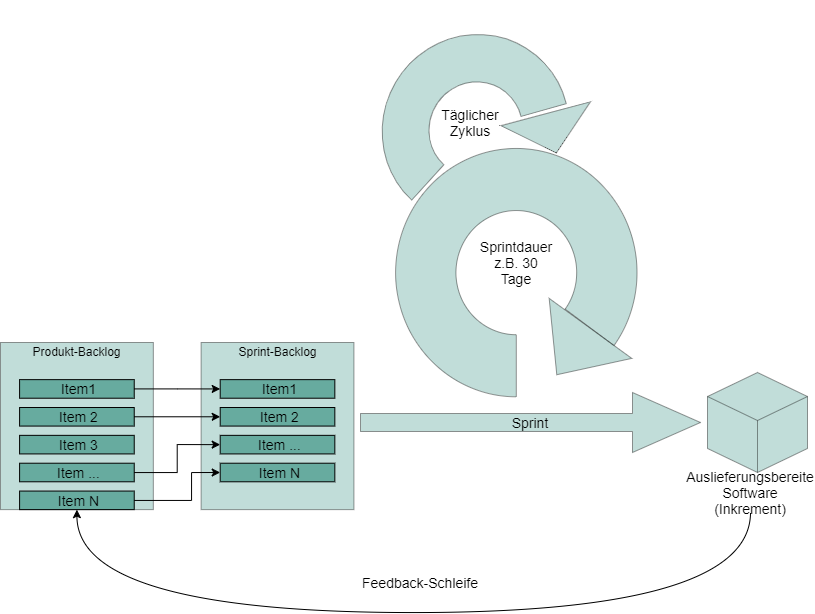
\includegraphics[width=0.8\textwidth]{Grafiken/SCRUM.png}
    \captionof{figure}{Ablauf des SCRUM-Modells}
    \label{Grafik:Ablauf des SCRUM-Modells}
\end{center}

Damit dieser vergleichsweise aufwändige Ablauf erfolgreich in der Praxis umgesetzt werden kann, setzt \gls{SCRUM} insbesondere auf zwischenmenschliche Kommunikation und Werte. Hierzu zählen insbesondere Offenheit, ein hohes Maß an Autonomie für die einzelnen Mitarbeiter, Transparent und Stringenz in den Abläufen \cite{SCRUM_values_nodate}.\newline
Ein weiterer, prominenter Vertreter ist das in seinen Abläufen stark an das Spiralmodell angelehnte Extreme Programming (\acrshort{XP}). Erstmalig im Jahr 2000 von Kent Beck niedergeschrieben \cite{beck_extreme_2000}, etabliert \acrshort{XP} 14 Prinzipien, mit denen bewährte Methoden \glqq im Extremen\grqq{} betrieben, also im großen Maßstab eingesetzt werden sollen.
Kent Beck war ebenfalls Mitautor des agilen Manifests, dementsprechend finden sich viele dieser Ideen im Extreme Programming wieder. Dazu gehören insbesondere die Fokussierung auf den Faktor Mensch, d.h. kollaboratives und gemeinsames Zusammenarbeiten bei gleichzeitiger Beibehaltung eines einheitlichen Tempos und Fehlertoleranz sind Teil dieser zentralen Prinzipien (vergleichbar mit der Zusammenarbeit innerhalb der \gls{SCRUM}-Teams). Zudem liegt der Fokus auf möglichst kleinen, nachvollziehbaren Entwicklungsschritten, also einer hohen Anzahl Iterationen. Dahinter steht die Annahme, dass viele Iterationen zu insgesamt höherer Code-Qualität und einem hohen Anteil wiederverwendbaren Codes führen (Vgl. \glqq{}[...]die Kunst, die Menge nicht getaner Arbeit zu maximieren [...]\grqq{} \cite{beck_manifest_2001}) Die nachfolgende Grafik verdeutlicht diese Zusammenhänge:

\begin{center}
    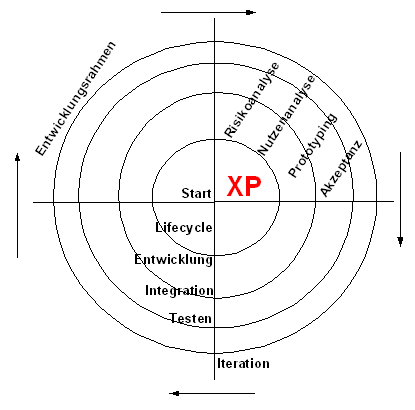
\includegraphics[width=0.6\textwidth]{Grafiken/XP-Life.png}
    \captionof{figure}{Zyklen des Extreme Programmings \cite{huttermann_xp_2006}}
    \label{Grafik:Zyklen des Extreme Programmings}
\end{center}

Zusammenfassend kann man festhalten, dass agile Softwareentwicklung und Softwareentwicklungsmodelle durch die folgenden Merkmale gekennzeichnet sind (in Anlehnung an \cite{moniruzzaman2013comparative} nach \cite{goos_extreme_2002}):
\begin{itemize}
    \item iterativ / wiederholend
    \item inkrementell / fortschreitend (das fertige Produkt wird nicht in einem Schritt erstellt)
    \item selbstorganisierend (insbesondere die Projektteams untereinander)
    \item aufstrebend (\glqq{}emergent\grqq{}), lernen also aus ihren eigenen Abläufen
\end{itemize}
Vor dem Hintergrund der vielen variablen Prozessbestandteile ist es wichtig zu beachten, dass agil ungleich beliebig ist.
Agile Softwareentwicklung kann erheblich einfacher auf wechselnde Anforderung reagieren als monolithische Modelle, trotzdem sind definierte Abläufe nicht änderbar. Änderungen sind nur an definierten Punkten möglich und agile Softwareentwicklung bedeutet daher nie unbegrenzte Flexibilität. 
\subsection{DevOps und CI/CD}
% \addcontentsline{toc}{subsection}{DevOps und CI/CD}
\label{DevOps und CI/CD}
\gls{DevOps} ist der Ansatz der agilen Softwareentwicklung, weitergedacht in den Betriebsalltag einer Software. \gls{DevOps} selbst ist ein Kunstwort aus \glqq{}Development\grqq{} und \glqq{}Operations\grqq{}. \gls{DevOps} bezeichnet die direkte Integration von Unternehmenskultur und unterstützender \acrshort{IT}-Prozesse in den Softwareentwicklungsprozess \cite{halstenberg_devops_2020}. Diese unterstützenden \acrshort{IT}-Prozesse umfassen oftmals Aufgaben, wie Bereitstellung der Umgebung für den Test- und Wirkbetrieb einer Software, Verfügbarmachung einer Software für den Endkunden und Betreuung der Anwendung im Alltag oder auch Qualitätssicherung \cite{DevOps_Definition_AWS}. \gls{DevOps} soll dabei die Entwicklung und Bereitstellung von Software erleichtern und die damit verbundene Time-to-Market (Bereitstellungszeit) erheblich verkürzen. Gleichzeitig dienen diese Vorteile auch der Unterstützung anderer Phasen im Softwarelebenszyklus, insbesondere dem Patch-Management und der Wartung \cite{DevOps_Definition_Microsoft}.\newline
\gls{DevOps} ist dabei mehr als nur ein Neuordnen vorhandener Abläufe. Der Ansatz umfasst nicht nur technische Änderungen, sondern Änderungen der gesamten Unternehmenskultur: Vorher getrennte Abläufe werden miteinander vernetzt und vorher getrennte Zuständigkeiten entfallen. Abteilungen und Organisationseinheiten müssen nicht nur mehr miteinander kommunizieren, sondern müssen füreinander transparent sein. Zudem erhalten sie untereinander Einblick in Prozesse und Gebiete, für die sie eigentlich nicht zuständig sind \cite{DevOps_Definition_Microsoft} \cite{DevOps_Definition_AWS}.\newline
Vor diesem Hintergrund sind die Schlagworte \glqq{}Continuous Development\grqq{} und \glqq{}Continuous Integration\grqq{} Ausprägungen der \gls{DevOps}-Philosophie. Continuous Development (\acrshort{CD}) bezeichnet den iterativ-inkrementellen Ansatz der Softwareentwicklung, der allen agilen Modellen und damit auch dem \gls{DevOps}-Ansatz zugrunde liegt. Dabei geht es um die permanente und zyklische Weiterentwicklung der Code-Basis einer Software. Continuous Integration (\acrshort{CI}) bezeichnet die dabei stattfindende, fortlaufende Integration von Änderungen und Erweiterungen in die bestehenden Anwendungen. \acrshort{CD} verfügt aber noch über eine weitere Bedeutung: Continuous Delivery. Delivery, also die Auslieferung oder Bereitstellung der Software, kann sich dabei auf die Bereitstellung des fertigen Produktes, z.B. in Form eines Datenträgers oder Installationsimages, beschränken. Der Ansatz kann aber auch erheblich weitergedacht werden. Dadurch sind Szenarien möglich, bei denen eine Änderung in einer direkten Kette vom ausführenden Programmierer über die Versionsverwaltung, Build-Umgebung, Test-Umgebung und Bereitstellung direkt in ein Produktivsystem im eigenen Unternehmen oder bei einem Kunden geladen wird. Diese Kette wird als \acrshort{CI}/\acrshort{CD}-Pipeline bezeichnet \cite{DevOps_Definition_Microsoft}  \cite{DevOps_Definition_AWS} \cite{atlassian_CivsCDvsCD_nodate} \cite{NodeRed_CICD_nodate}. 

% 4.
\section{Potenziale von CI/CD}
% \addcontentsline{toc}{section}{Potenziale von CI/CD}
\label{Potenziale von CI/CD}
Der nachfolgende Abschnitt betrachtet die Potenziale, die der Einsatz von \acrshort{CI}/\acrshort{CD} sowohl aus betriebswirtschaftlicher als auch aus technischer Sicht bietet.
\subsection{Betriebswirtschaftliche Potenziale}
% \addcontentsline{toc}{subsection}{Betriebswirtschaftliche Potenziale}
\label{Betriebswirtschaftliche Potenziale}
Lorem Ipsum
\subsection{Technische Potenziale}
% \addcontentsline{toc}{subsection}{Technische Potenziale}
\label{Technische Potenziale}
Ebenso wie betriebswirtschaftliche Potenziale, bietet eine \gls{DevOps}-Kultur auch technische Vorteile. Dies umfasst auch Erleichterungen für die technischen Mitarbeiter, wie Programmierer oder Administratoren. \gls{DevOps} hat einen stark Mensch-bezogenen Ansatz in seinen Grundsätzen des offenen und gleichberechtigen Zusammenarbeitens. Integraler Bestandteil von \gls{DevOps} ist das Auflösen von \glqq{}Silos\grqq{} \cite{leite_survey_2020}, also Bastionen begrenzten Wissens. Dieser kollaborative Ansatz bietet für Mitarbeiter einerseits die Möglichkeit neue Erfahrungen zu sammeln und Interessen an Themen jenseits des eigenen Fachbereiches auszuleben \cite{leite_survey_2020}. Da \gls{DevOps} zeitgleich auf die Grundgedanken des agilen Manifests zurückgeht, ist die Idee regelmäßiger Arbeitszeiten und der Vermeidung exzessiver Belastung an einzelnen Stellen immanent (Vgl. \glqq{}gleichmäßiges Tempo\grqq{}, \ref{Betriebswirtschaftliche Potenziale}).
Zeitgleich entlastet \acrshort{CI}/\acrshort{CD} über den Grad der Automatisierung und die Art der Architektur die einzelnen Entwickler: Software muss so gebaut sein, dass sie in Teilen iterativ verändert werden kann, ohne Auswirkungen auf das Gesamtprojekt zu haben (\glqq{}Microservice\grqq{} \cite[S. 14]{leite_survey_2020}). Die dadurch in die Software eingebrachte Modularität macht es nicht mehr erforderlich jede Facette eines Projektes zu kennen. Änderungen am Code werden dadurch einfacher und die Einstiegshürden für neue oder fachfremde Entwickler geringer. Dies betrifft ebenfalls den notwendigen Aufwand zur Fehlersuche und -beseitigung (Bugfixing) \cite{hilton_usage_2016}.

% //Todo
% zhao_impact_2017
% rahman_characterizing_2018

% 5.
\section{UseCases aus der Praxis}
% \addcontentsline{toc}{section}{UseCases aus der Praxis}
\label{UseCases aus der Praxis}
Die nachfolgenden Abschnitte stellen exemplarisch Tools und Anwendungfällebieten (UseCases) zu \acrshort{CI}/\acrshort{CD} aus der Praxis vor. Dabei wird eine Unterscheidung zwischen Anwendungsfällen, in denen proprietäre Lösungen und Anwendungsfällen, in denen Opensource-Lösungen zum Einsatz kommen, getroffen. Diese Unterscheidung ist der Bandbreite an möglichen Lösungen und Tools geschuldet. U.a. umfassen die proprietären Lösungen auch die (fast) vollautomatisierten Cloudplattformen von Amazon (\acrshort{AWS}) und Microsoft (Azure).
\subsection{Microsoft Azure}
% \addcontentsline{toc}{subsection}{Microsoft Azure}
\label{Microsoft Azure}
\subsection{Amazon Web Services}
% \addcontentsline{toc}{subsection}{Amazon Web Services}
\label{Amazon Web Services}
\subsection{OpenSource-Tools}
% \addcontentsline{toc}{subsection}{OpenSource-Tools}
\label{OpenSource-Tools}

% 6.
\section{Benötigte Funktionen für eine CI/CD-Pipeline}
% \addcontentsline{toc}{section}{Benötigte Funktionen für eine CI/CD-Pipeline}
\label{Benoetigte Funktionen für eine CI/CD-Pipeline}
Die vorangegangenen Abschnitte haben einen Eindruck vermittelt, wie langwierig der Weg von klassischer über agile Softwareentwicklung hin zu \gls{DevOps} und \acrshort{CI}/\acrshort{CD} war. Die Abschnitte \ref{UseCases mit proprietärer Software}  und \ref{UseCases mit Opensource-Software} haben einen Eindruck vermittelt, welche Vielzahl von Anwendungen es in diesem weiten Themenfeld gibt. Abschließend ist nun zu betrachten, welche Elemente zwischen den Lösungen gleich und damit integraler Bestandteil einer \acrshort{CI}/\acrshort{CD}-Pipeline sind.\newline
Eine \acrshort{CI}/\acrshort{CD}-Pipeline \glqq{}verbindet\grqq{} die folgenden Entwicklungsphasen miteinander (In Anlehnung an \cite{redhat_cicd_pipline} und \cite{meyer_continuous_2014}):
\begin{enumerate}
    \item Continuous Integration
    \begin{enumerate}
        \item Erstellen / Entwicklung
        \item Test (lokal)
        \item Zusammenführen (mit dem Rest der Code-Basis, \glqq{}Merging\grqq{})
    \end{enumerate}
    \item Continuous Delivery
        \begin{enumerate}
        \item Bereitstellung
        \item Automatische Veröffentlichung 
    \end{enumerate}
    \item Continuous Deployment
        \begin{enumerate}
        \item Bereitstellung in Zielumgebung
        \item Zielumgebung kann lokal oder entfernt (remote) im eigenen Unternehmen oder beim Kunden sein
    \end{enumerate}
\end{enumerate}
Aus diesem Ablauf ergeben sich die folgenden Elemente, die in einem derartigen Ablauf notwendig sein:
% !h um die automatische Anordnung am Seitenanfang zu unterdrücken
% https://de.overleaf.com/learn/latex/Tables#Positioning_tables
% \begin{table]} ... \end{table} damit diese Tabelle im Tabellenverzeichnis aufgenommen wird
% Landscape für Querausrichtung der Tabelle
    \begin{table}[!h]
        \centering
        \begin{tabular}{|p{2cm}|p{4cm}|p{8cm}|}
            \hline
            Abschnitt & Phase & Tool\\
            \hline
            Continuous Integration & Entwicklung & Lokale \acrshort{IDE}, (verteiltes) Versionskontrollsystem z.B. Git\\
            \hline
            Continuous Integration & Test & Lokaler Compiler / Interpreter der jeweiligen Sprache, lokale Tests\\
            \hline
            Continuous Integration & Zusammenführen (Merge) & (verteiltes) Versionskontrollsystem z.B. Git\\
            \hline
            Continuous Delivery & Release & Buildserver z.B. Jenkins\\
            \hline
            Continuous Delivery & Bereitstellung & Repository / Versionsverwaltung für die fertige Software, z.B. Nexus \cite{zanini_integrating_2018}\\
            \hline
            Continuous Deployment & Rollout in Test- oder Produktivumgebung & Softwareorchestrierungstool\\
            \hline
        \end{tabular}
            \caption{Phasen und Elemente einer \acrshort{CI}/\acrshort{CD}-Pipeline}
            \label{Tabelle:Phasen und Elemente einer CICD-Pipeline}
    \end{table}
\newline
Diese relativ kurze Liste der notwendigen Voraussetzungen ist einerseits bewusst vereinfachend gehalten, zeigt aber andererseits auch, mit wie wenigen Tools eine \acrshort{CI}/\acrshort{CD}-Pipeline etabliert werden kann. Aufgrund der vereinfachenden Darstellung ist auch davon auszugehen, das reale Implementierungen von \acrshort{CI}/\acrshort{CD}-Pipelines entsprechend komplexer sind.
\newline

7.
\section{Fazit}
% \addcontentsline{toc}{section}{Fazit}
\label{Fazit}


% Anhang / Backmatter
\clearpage

% Römische Seitennummerierung
\pagenumbering{roman}
\setcounter{page}{9}

% Literaturverzeichnis
% Stil des Literaturverzeichnisses
% IEEEtran
\bibliographystyle{IEEEtran}
\bibliography{Inhalt/03Anhang/Literaturverzeichnis}

\clearpage

% Rechtsprechungsverzeichnis einfügen
% \include{Inhalt/03Anhang/Rechtsprechungsverzeichnis}

% Quellenverzeichnis einfügen
% \include{Inhalt/03Anhang/Quellenverzeichnis}

% Deutschsprachige ehrenwörtliche Erklärung einfügen
\section*{Ehrenwörtliche Erklärung}
\addcontentsline{toc}{section}{Ehrenwörtliche Erklärung}
Hiermit versichere ich, dass die vorliegende Arbeit von mir selbstständig und ohne unerlaubte Hilfe angefertigt worden ist, insbesondere dass ich alle Stellen, die wörtlich oder annähernd wörtlich aus Veröffentlichungen entnommen sind, durch Zitate als solche gekennzeichnet habe. Ich versichere auch, dass die von mir eingereichte schriftliche Version mit der digitalen Version übereinstimmt. Weiterhin erkläre ich, dass die Arbeit in gleicher oder ähnlicher Form noch keiner Prüfungsbehörde/Prüfungsstelle vorgelegen hat. Ich erkläre mich damit einverstanden/nicht einverstanden, dass die Arbeit der Öffentlichkeit zugänglich gemacht wird. Ich erkläre mich damit einverstanden, dass die Digitalversion dieser Arbeit zwecks Plagiatsprüfung auf die Server externer Anbieter hochgeladen werden darf. Die Plagiatsprüfung stellt keine Zurverfügungstellung für die Öffentlichkeit dar.

\vspace{2cm}
\begin{tabularx}{\textwidth}[b]{p{5cm} X p{5cm}} \cline{1-1} \cline{3-3}
(Ort, Datum)  & & Unterschrift Danny Langenbach
\end{tabularx}

% Englischsprachhige ehrenwörtliche Erklärung einfügen
% \section*{Declaration in lieu of oath}
\addcontentsline{toc}{section}{Declaration in lieu of oath}
I hereby declare that I produced the submitted paper with no assistance from any other party and without the use of any unauthorized aids and, in particular, that I have marked as quotations all passages, which are reproduced verbatim or nearby-verbatim from publications. Also, I declare that the submitted print version of this thesis is identical with its digital version. Further, I declare that this thesis has never been submitted before to any examination board in either its present form or in any other sim-ilar version. I herewith agree\sout{/disagree} that this thesis may be published. I herewith consent that this thesis may be uploaded to the server of external contractors for the purpose of submitting it to the contractors’ plagiarism detection systems. Uploading this thesis for the purpose of submitting it to plagiarism detection systems is not a form of publication.

\vspace{2cm}
\begin{tabularx}{\textwidth}[b]{p{5cm} X p{5cm}} \cline{1-1} \cline{3-3}
(Location, date)  & & (genuine signature) Danny Langenbach
\end{tabularx}

\end{document}